\section{Introduction}\label{sec:intro}

%Intro
%Reason for image colorization
%
%Types of image colorization (from literature review, but shorter?)
%by example
%by user input
%by a trained machine
%
%Research problem: 
%how to colorize an image using NN
%How to pick a color: mean in color space is sepia
%
%What is in the rest of this paper


\IEEEPARstart{I}{n} this paper several approaches to using a deep neural network to colorize grayscale images are compared. Specifically, given grayscale image, the neural network can generate all the data needed to present a color version of the same image, without input of the user. 

There is a substantial amount of grayscale photographic material, from before the advent of the color camera. Color images may have a greater psychological impact on people than their grayscale counterparts.
In addition, automation of the colorization process can be applied in real time to grayscale video. Specifically (infra-red) surveillance cameras often save video in grayscale format. With the automated colorization techniques it may be possible to generate real-time color video, such that a human may more quickly understand what is seen in a video, in addition to a decrease in file size. In order to do this, it is required that the algorithm can colorize an image without intervention of a human.\\

As will be explained below, non-machine learning techniques are available for automatic image colorization. However, the drawback of these techniques is that they require either an image comparable to the grayscale image in terms of content, or user input on what color to use for different parts of the image. 
While this makes things much easier than the hand-made solution with photo editing software, it still requires a human to specify these inputs, which in turn disallows a real-time solution. This makes the case for a trained machine (i.e. neural network), which uses pre-supplied training data to learn, and while actually colorizing an image does not require additional input from a human.

Identified by the types of input required for colorization, there are three approaches to make the computer convert a grayscale image to a color image. Every approach uses the texture and intensity gradients present in the image to link a part of an image to either a learned or specified color. The three approaches are as follows:

\textbf{Colorize by example:} Image colorization can be performed by using a color image that is related to the grayscale image, in the sense that it contains similar objects with similar colors. The patterns in the color image are compared to those in the grayscale image, directly linking colors to the grayscale patterns and finding equal patterns in the to be colorized grayscale image. 
For example: to colorize a grayscale image of a zebra in a Savannah, another image of a zebra in a Savannah is required. The more comparable the image, the better the result is. This method is used in \cite{Charpiat}, \cite{Gupta} and \cite{Zheng}.

\textbf{Colorize by user input:} In this approach, the user specifies the color of different parts of the image by hand. While this is quite labor intensive, it guarantees that correct colors are used for the different segments in an image. 
As opposed to the \textit{colorize by example} method, this method cannot colorize images incorrectly purely based on similarity between contrast patterns. However, if the user does not know the original colors of the grayscale image, colorization is not possible. This method is used in \cite{Horiuchi} and \cite{Levin}.

\textbf{Colorize using a trained machine:} Techniques like convolutional neural networks allow training of a machine to recognize specific patterns in an image and coupling the recognized pattern to a color. This requires supplying the machine with training images of which both grayscale and color versions are available. 
After the training of the machine is completed, no human is needed to colorize an image since all information needed is contained within the system. This leads to a vast decrease in time consumption during colorization. One of the biggest downsides of this method is that objects are colorized based on experience with different objects of the same class. 
However, not all objects can be colorized purely based on their class of object, i.e. an object of class ``car" can have multiple colors, and during training multiple of these colors are shown to the machine, leading to an ambiguous mapping between object and color. The neural network method is used in \cite{Cheng}, \cite{Ho}, \cite{Krizhevsky} and \cite{Dahl}.\\

The research presented in this paper dives into how to best colorize an image using a Convolutional Neural Network (CNN). The question as to what is actually the best colorization of an image does not have one final answer. 
One answer could be that the best colorization would be the one that most people would be unable to distinguish from the original color image. This immediately involves the opinion of a human, warranting for example the use of a version of the Turing test, where for both ground truth color image and colorized image are shown to a human. The human in turn needs to pick which it thinks is colorized and which is the original. 
Although this makes quantification of the quality possible, it is labor intensive and a direct (mathematical) link between the way the system colorizes an image and result quality is not apparent. This makes it impossible to use for any gradient-based method of training the neural network. 

\begin{wrapfigure}{R}{0.37\textwidth}
	\vspace{-20pt}
	\begin{center}
		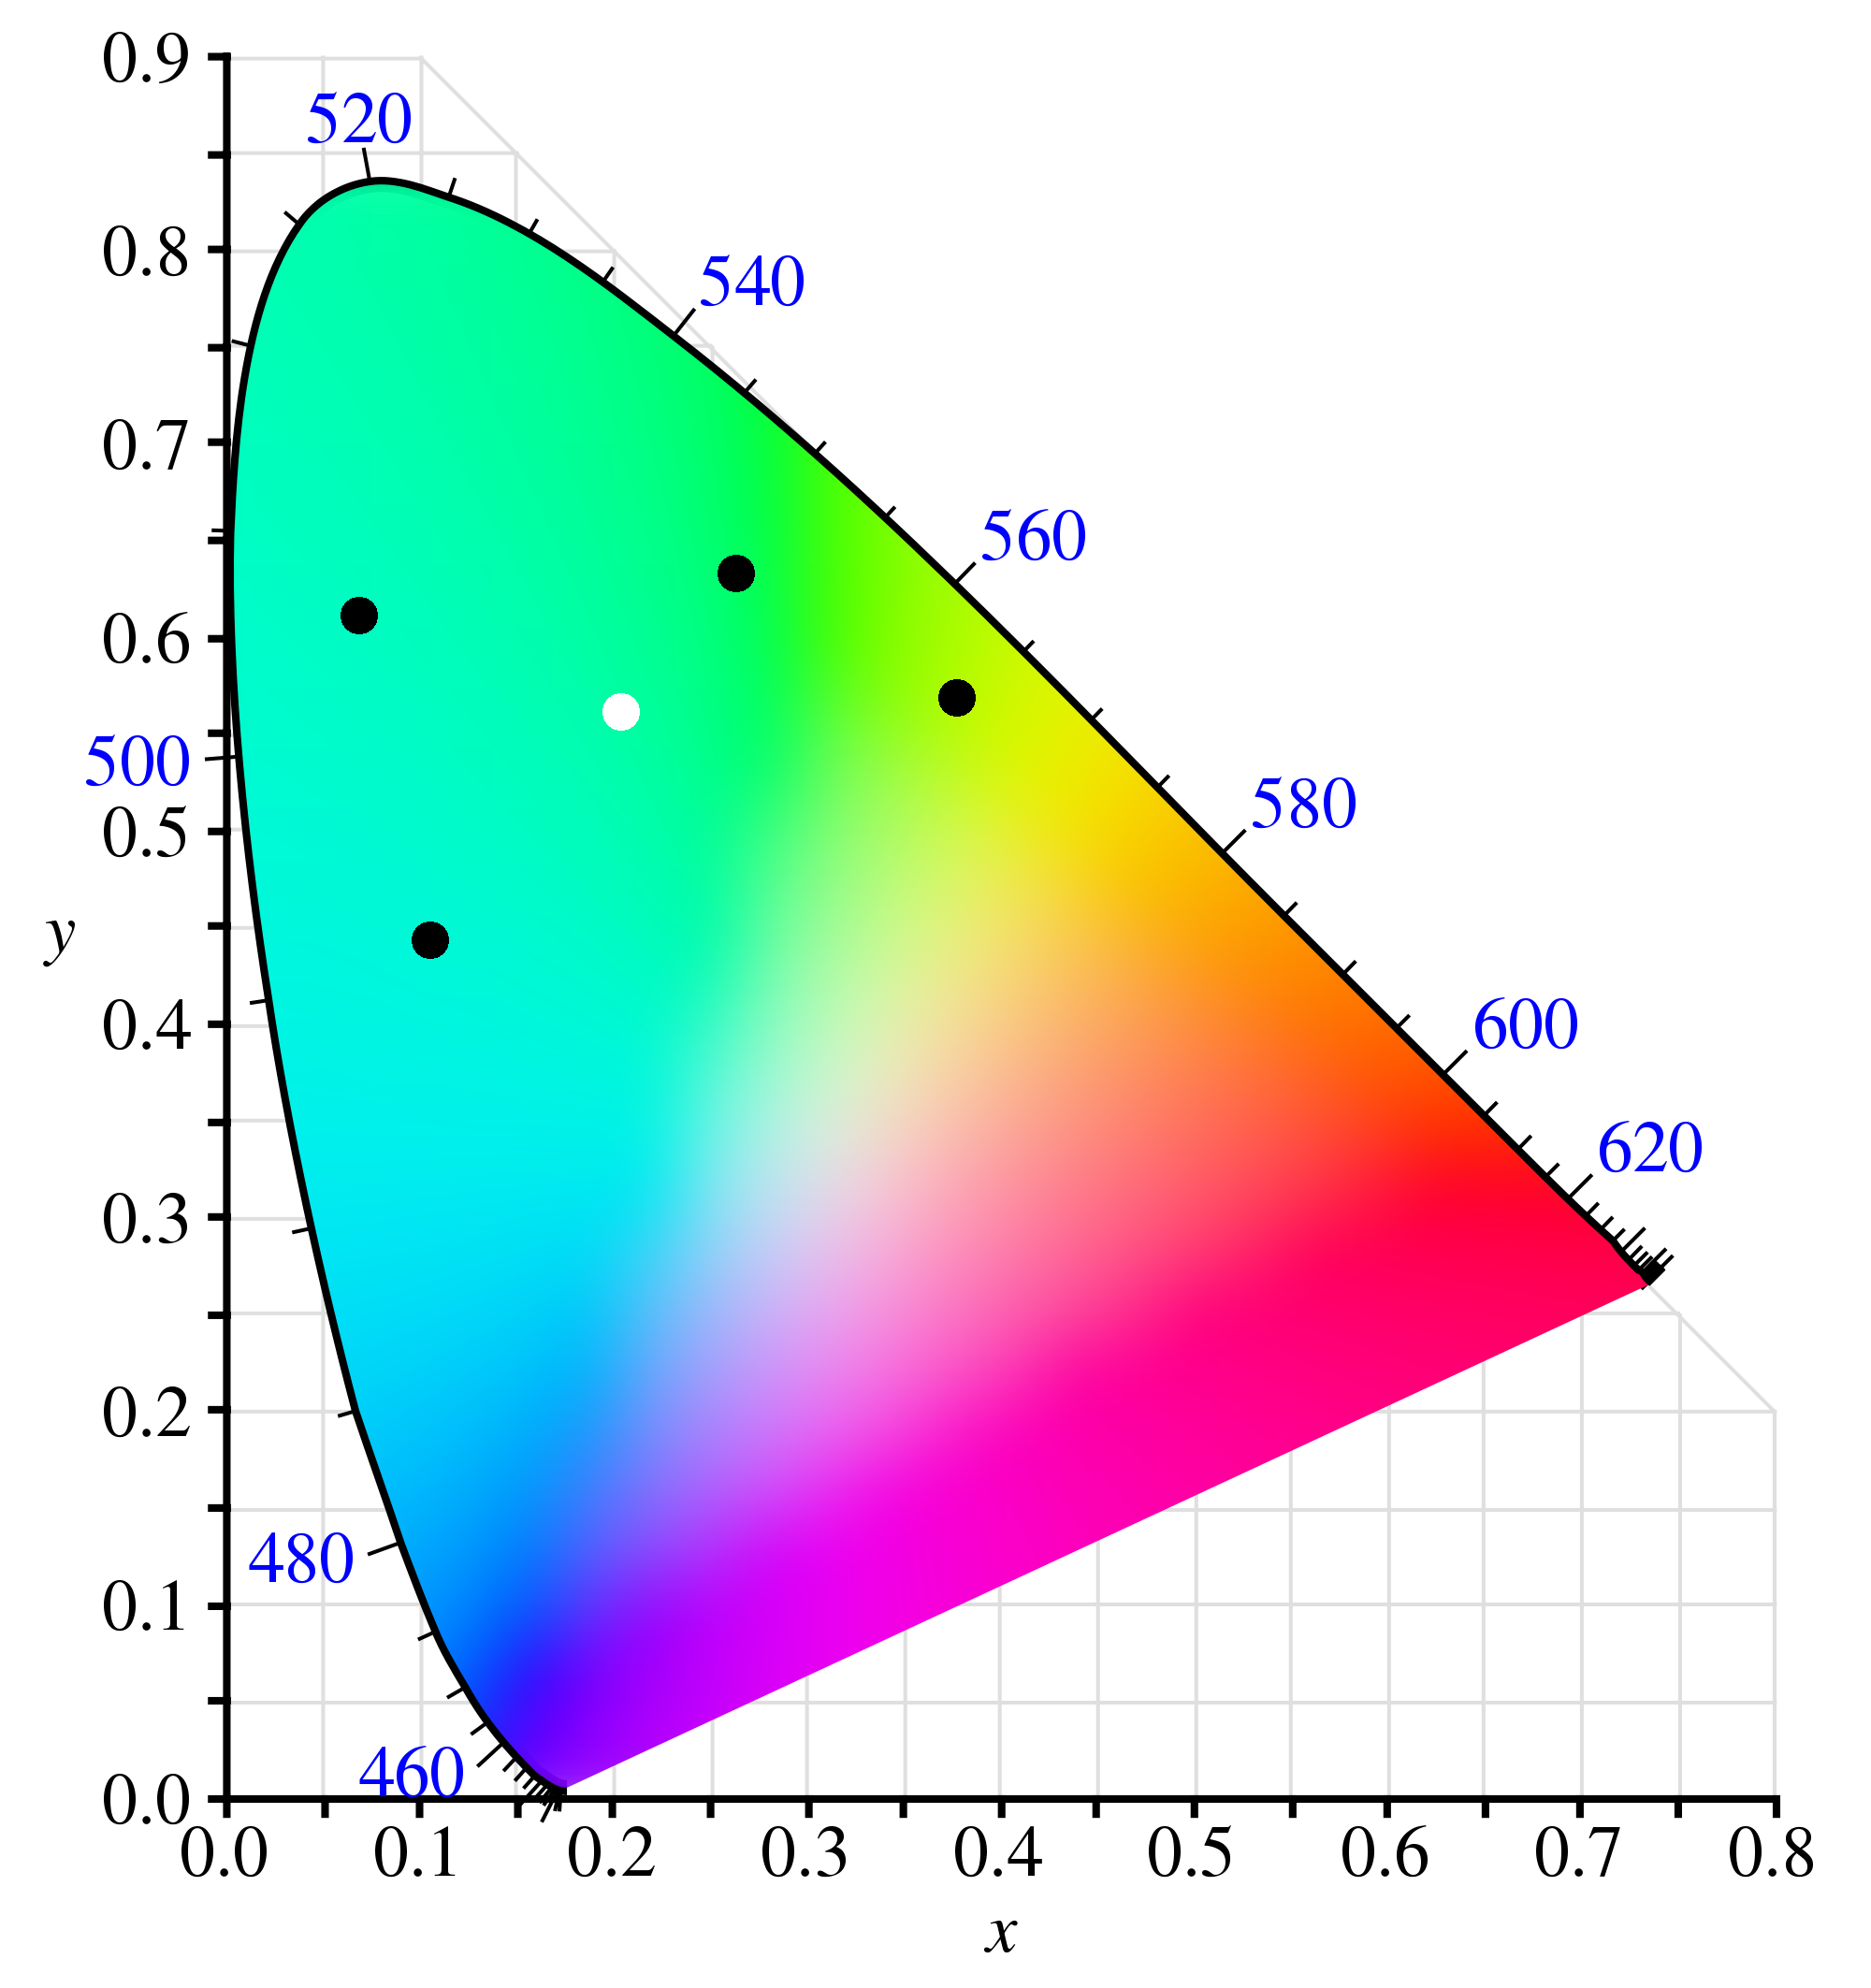
\includegraphics[width=0.37\textwidth]{saturation.png}
	\end{center}
	\caption{\label{fig:colorspacesaturation} The CIE 1931 color space containing all colors detectable by a human. When training a network to colorize to certain target colors of a green/blue object (black dots in image) minimizing the sum squared error, an average color will result (white dot in image), which most of the time leads to a less saturated color, i.e. more to the center of this color space. When the original colors are even more scattered, for example cars or clothes which do not inherently have a single color, a generic sepia color usually results.}
	\vspace{-20pt}
\end{wrapfigure}

Another way is to mathematically define a quality measure, probably involving the ground truth color image and the colorized image, putting a number to the difference between these two. 
One of the most used error measures is the sum of the squared errors, calculating the difference in color per pixel, squaring every individual component and summing to obtain the final measure. 
This approach is natural to start with, but leads to one of the biggest unsolved problems encountered in automatic image colorization: the averaging problem.

The averaging problem arises from the following: a neural network is shown numerous examples of a certain object, of which it needs to deduce color from a grayscale image of this object. 
A trained neural network, in order to have the lowest possible cumulative error for all the training images, is encouraged to take some sort of mean color of all examples of the object in the training data set, which leads to the lowest mean squared error. For most objects that are linked to a certain color (such as bricks or a cloudless sky), this leads to undersaturated results, as illustrated in figure \ref{fig:colorspacesaturation}. 
For objects that are not inherently linked to a certain color, this leads to a mean that lies somewhere in the center of the color space, which in practice often leads to a generic sepia tone\cite{Dahl}.\\
	
In the rest of the paper the research is detailed on the problem of automatic image colorization using neural networks, starting with a literature review containing relevant other neural networks in section \ref{sec:litreview}. Multiple ideas are derived from these previous works. In section \ref{sec:method} these ideas in combination with new insights are described, detailing the method and different architectures to try. After that the results, a discussion of the results, a conclusion and recommendations are given.
	
	




